\section{Exercise 3}

\begin{frame}{Exercise 3: Standardization}
    \begin{tikzpicture}
        \node[] at (-5.25, -3.5) {};
        \node[] at (5.25, 3.5) {};

        \only<1-2>{
            \node[text width=10cm, align=flush center, font=\bfseries] at (0, 1) {Why do we standardize the validation set based on information from the training set?};
        }
        \only<2>{
            \node[text width=10cm] at (0, -0.2) {
                \begin{itemize}
                    \item To avoid data leakage
                    \item To minimize the impact of distributional differences
                \end{itemize}
            };
        }
        \only<3-6>{
            \node[label=above:\footnotesize{Train}, inner sep=0pt] (train) at (-3, 1.5) {
                \begin{tabular}{|c|c|}
                    \hline
                    \textbf{x}&\textbf{y}\\
                    \hline
                    -1&1.1\\
                    \alert<4-6>{1}&\alert<4-6>{1.5}\\
                    3&1.7\\
                    \hline
                \end{tabular}
            };
            \node[label=above:\footnotesize{Validation}, inner sep=0pt] (val) at (3, 1.5) {
                \begin{tabular}{|c|c|}
                    \hline
                    \textbf{x}&\textbf{y}\\
                    \hline
                    2&1.9\\
                    \alert<4>{1}&\alert<4>{1.5}\\
                    5&2.4\\
                    \hline
                \end{tabular}
            };
        }
        \only<5-6>{
            \node[inner sep=0pt] (trainstd) at (-3, -1.5) {
                \begin{tabular}{|c|c|}
                    \hline
                    \textbf{x}&\textbf{y}\\
                    \hline
                    -1.22&1.1\\
                    \alert<6>{0}&\alert<6>{1.5}\\
                    1.22&1.7\\
                    \hline
                \end{tabular}
            };
            \node[inner sep=0pt] (valstd) at (3, -1.5) {
                \begin{tabular}{|c|c|}
                    \hline
                    \textbf{x}&\textbf{y}\\
                    \hline
                    -0.39&1.9\\
                    \alert<6>{-0.98}&\alert<6>{1.5}\\
                    1.37&2.4\\
                    \hline
                \end{tabular}
            };
            \draw[-stealth] (train) -- (trainstd);
            \draw[-stealth] (val) -- (valstd);
        }
    \end{tikzpicture}
\end{frame}

\begin{frame}{Exercise 3: Solution}
    \centering
    \vfill
    \scriptsize{\url{http://localhost:8888/notebooks/notebooks/Solution\%203.ipynb}}
    \vfill
\end{frame}
